% !TeX root = writeup.tex 

\section{Problem Setting}
\label{sec:problem setting }
\label{sec:models_and_notation}
We consider two \emph{groups} $\popa$ and $\popb$, which comprise a $\fraca$ and $\fracb = 1 - \fraca$ fraction of the total population, and an \emph{institution} which makes a binary decision for each individual in each group, called \emph{selection}. 
Individuals in each group are assigned \emph{scores} in $\calX := [\maxscore]$, 
and the scores for group $\popj \in \{\popa,\popb\}$ are distributed according $\dist\supj \in \Simplex$. 
The institution selects a \emph{policy} $\pol:=(\pol\supa,\pol\supb)\in[0,1]^{2\maxscore}$, where $\pol\supj(x)$ corresponds to the probability the institution selects an individual in group $\popj$ with score $x$. 
One should think of a score as an abstract quantity which summarizes how well an individual is suited to being selected; examples are provided at the end of this section.

We assume that the institution is utility-maximizing, but may impose certain constraints to ensure that the policy $\pol$ is \emph{fair}, in a sense described in Section~\ref{sec:fairness_criteria}. We assume that there exists a function $\util: \maxscore \to \R$, such that the institution's expected utility for a policy $\pol$ is given by 
\begin{eqnarray}
\textstyle
\label{eqn:inst_util}
\Util(\pol) = \sum_{\popj \in \pops } g_{\popj}\sum_{x \in \X} \polj(x)\distj(x)\util(x).
\end{eqnarray}
%We denote the mean score of subpopulations by $\mean\supa:= \sum_{x \in \X} x \cdot \dst\supa,~ \mean\supb:= \sum_{x \in \X} x \cdot \dst\supb$.
Novel to this work, we focus on the effect of the selection policy $\pol$ on the groups $\popa$ and $\popb$. 
We quantify these \emph{outcomes} in terms of an average effect that a policy $\polj$ has on group $\popj$. Formally, for a function $\chg(x):\X \to \R$, we define the average change of the mean score $\mean\supj$ for group $\popj$ 
\begin{eqnarray}
\textstyle
\label{eqn:delmean}
\delmean\supj (\pol) := \sum_{x \in \X} \dst\supj(x)\pol\supj(x)\chg(x) \:. 
\end{eqnarray}
We remark that many of our results also go through if $\delmean\supj(\pol)$ simply refers to an abstract change in well-being, not necessarily a change in the mean score. Furthermore, it is possible to modify the definition of $\delmean\supj(\pol)$ such that it directly considers outcomes of those who are not selected.\footnote{\label{footnote:negative_dec_outcomes}
If we consider functions $\chg_p(x):\X \to \R$ and $\chg_n(x):\X \to \R$ to represent the average effect of selection and non-selection respectively, then $
\delmean\supj (\pol) := \sum_{x \in \X} \dst\supj(x) \left(\pol\supj(x)\chg_p(x) + (1-\pol\supj(x))\chg_n(x) \right)$.
This model corresponds to replacing $\chg(x)$ in the original outcome definition with $\chg_p(x)-\chg_n(x)$, and adding a offset $\sum_{x \in \X} \dst\supj(x)\chg_n(x)$. Under the assumption that $\chg_p(x)-\chg_n(x)$ increases in $x$, this model gives rise to outcomes curves resembling those in Figure~\ref{fig:outcome_curve} up to vertical translation. All presented results hold unchanged under the further assumption that $\delmean (\accrate^\maxprof) \geq 0$.
}
Lastly, we assume that the \emph{success} of an individual is independent of their group given the score; that is, the score summarizes all relevant information about the success event, so there exists a function $\pb:\X \to [0,1]$ such that individuals of score $x$ succeed with probability $\pb(x)$.

We now introduce the specific domain of credit scores as a running example in the rest of the paper, after which we present two more examples showing the general applicability of our formulation to many domains. 


\begin{exmp}[Credit scores] 
	\label{ex:credit_lending} In the setting of loans, scores $x \in [\maxscore]$ represent credit scores, and the bank serves as the institution. The bank chooses to grant or refuse loans to individuals according to a policy $\pol$. Both bank and personal utilities are given as functions of loan repayment, and therefore depend on the success probabilities $\pb(x)$, representing the probability that any individual with credit score $x$ can repay a loan within a fixed time frame. The expected utility to the bank is given by the expected return from a loan, which can be modeled as an affine function of $\pb(x)$: $\util(x) = u_+\pb(x) + u_-(1-\pb(x))$, where $u_+$ denotes the profit when loans are repaid and $u_-$ the loss when they are defaulted on. Individual outcomes of being granted a loan are based on whether or not an individual repays the loan, and a simple model for $\chg(x)$ may also be affine in $\pb(x)$: $\chg(x) = \cgood \pb(x) + \cbad (1 - \pb(x))$, modified accordingly at boundary states. The constant $c_+$ denotes the gain in credit score if loans are repaid and $c_-$ is the score penalty in case of default.
	% If an individual gets a loan, let $\cgood$ be the expected change in their score if they successfully repay, and let $\cbad$ that if they default. Then the simple individual utility function 
	% \begin{align}
	% \chg(x) = \cgood \pb(x) + \cbad (1 - \pb(x))~,
	% \end{align}
	% unless $x$ is the top or bottom state, in which case transitions are modified accordingly.
	
	% Note that in this example, the changes in state and utility result only from positive selection decisions (i.e. loans granted). That is, individuals who are not selected remain at their current state and correspond to zero utility on average. We can further define a drift process like drift-towards-current-mean to model population level interactions that occur in addition to loans. 
	
	
\end{exmp}


\begin{exmp}[Advertising]
	\label{ex:advertizing}
	A second illustrative example is given by the case of advertising agencies making decisions about which groups to target. An individual with product interest score $x$ responds positively to an ad with probability $\pb(x)$. The ad agency experiences utility $\util(x)$ related to click-through rates, which increases with $\pb(x)$. Individuals who see the ad but are uninterested may react negatively (becoming less interested in the product), and $\chg(x)$ encodes the interest change. 
	If the product is a  positive good like education or employment opportunities, interest can correspond to well-being.
	Thus the advertising agency's incentives to only show ads to individuals with extremely high interest may leave behind groups whose interest is lower on average. 
	A related historical example occurred in advertisements for computers in the 1980s, where male consumers were targeted over female consumers, arguably contributing to the current gender gap in computing. %\sarah{clean up this social implication reference}\\
\end{exmp}

\begin{exmp}[College Admissions]
	\label{ex:admissions}
	
	The scenario of college admissions or scholarship allotments can also be considered within our framework. Colleges may select certain applicants for acceptance according to a score $x$, which could be thought encode a ``college preparedness'' measure. The students who are admitted might ``succeed" (this could be interpreted as graduating, graduating with honors, finding a job placement, etc.) with some probability $\pb(x)$ depending on their preparedness. The college might experience a utility $\util(x)$ corresponding to alumni donations, or positive rating when a student succeeds; they might also show a drop in rating or a loss of invested scholarship money when a student is unsuccessful. The student's success in college will affect their later success, which could be modeled generally by $\chg(x)$. In this scenario, it is challenging to ensure that a single summary statistic $x$ captures enough information about a student; it may be more appropriate to consider $x$ as a vector as well as more complex forms of $\pb(x)$. 
\end{exmp}

While a variety of applications are modeled faithfully within our framework, there are limitations to the accuracy with which real-life phenomenon can be measured by strictly binary decisions and success probabilities. Such binary rules are necessary for the definition and execution of existing fairness criteria, (see Sec.~\ref{sec:fairness_criteria}) and as we will see, even modeling these facets of decision making as binary allows for complex and interesting behavior.


\subsection{The Outcome Curve}
\label{sec:pop_outcomes}
We now introduce important outcome regimes, stated in terms of the change in average group score. A policy $(\pola,\polb)$ is said to cause \emph{active harm} to group $\popj$ if $\delmean\supj(\pol\supj) < 0$, \emph{stagnation} if $\delmean\supj(\pol\supj) = 0$, and \emph{improvement} if $\delmean\supj(\pol\supj) > 0$. Under our model, $\maxprof$ policies can be chosen in a standard fashion which applies the same threshold $\pol^\maxprof$ for both groups, and is agnostic to the distributions $\dista$ and $\distb$.  Hence, if we define
\begin{eqnarray}
\delmean\supj^{\maxprof}:= \delmean\supj(\pol^\maxprof)
\end{eqnarray}
we say that a policy causes \emph{relative harm} to group $\popj$ if $\delmean\supj(\polj) < \delmean\supj^{\maxprof}$, and \emph{relative improvement} if $\delmean\supj(\polj) > \delmean\supj^{\maxprof}$. In particular, we focus on these outcomes for a disadvantaged group, and consider whether imposing a fairness constraint improves their outcomes relative to the $\maxprof$ strategy. From this point forward, we take $\popa$ to be disadvantaged or protected group. 

% to do: change textwidth to colwidth
\begin{figure*}
\begin{subfigure}{0.7\textwidth}
\centering
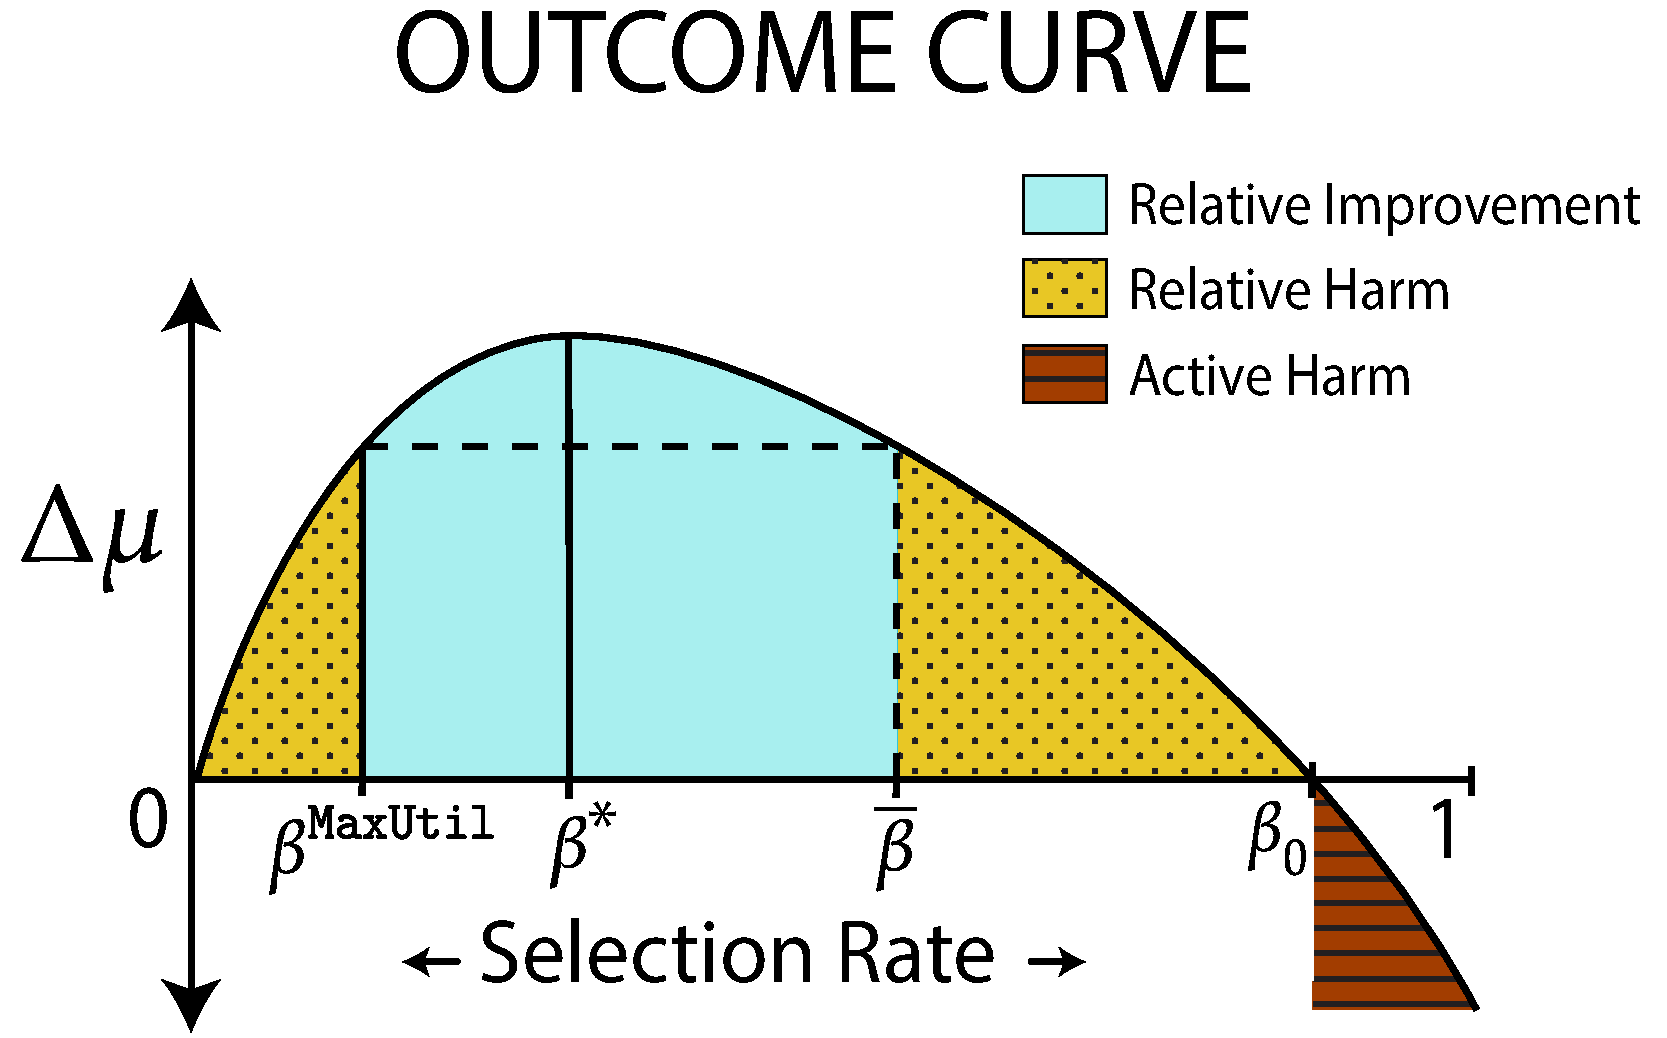
\includegraphics[width=\textwidth]{figures/outcome_curves/outcome_curve_full.pdf}
\caption{}
\label{subfig:outcome_region}
\end{subfigure}%
\begin{subfigure}{.3\textwidth}
\centering
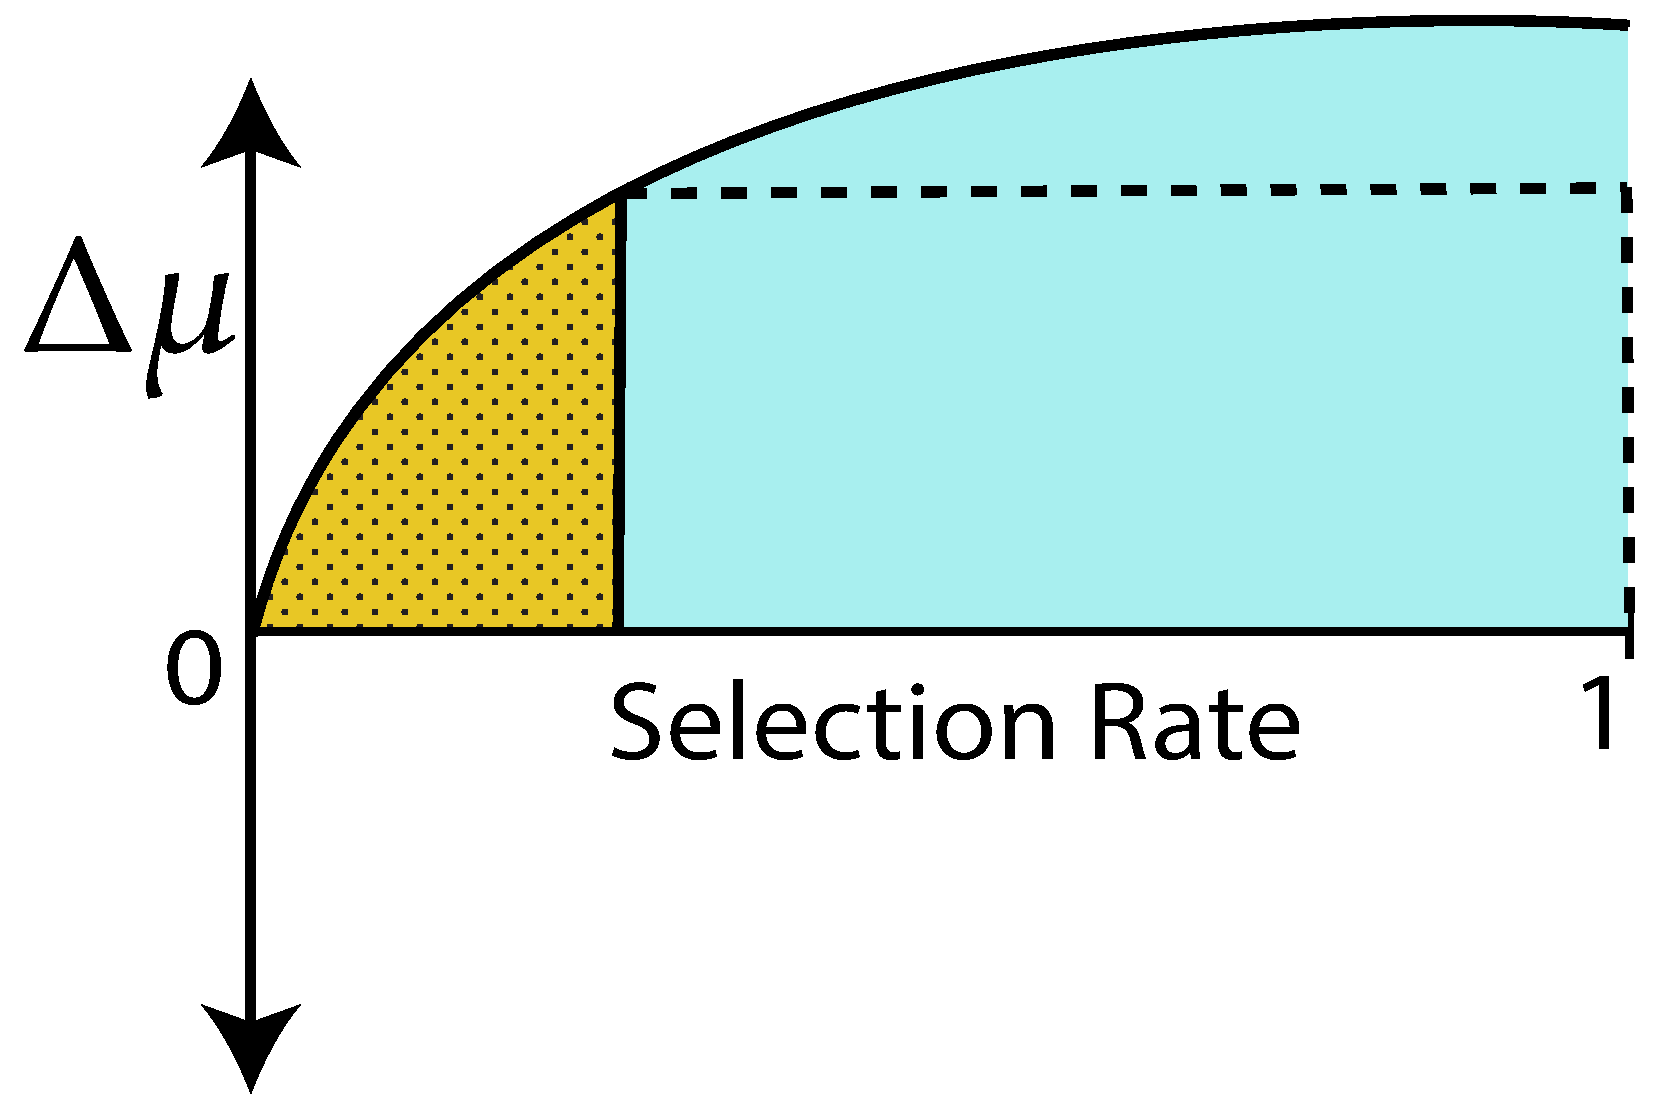
\includegraphics[width=\textwidth]{figures/outcome_curves/outcome_curve_great.pdf}
\caption{}
\label{fig:sub1}
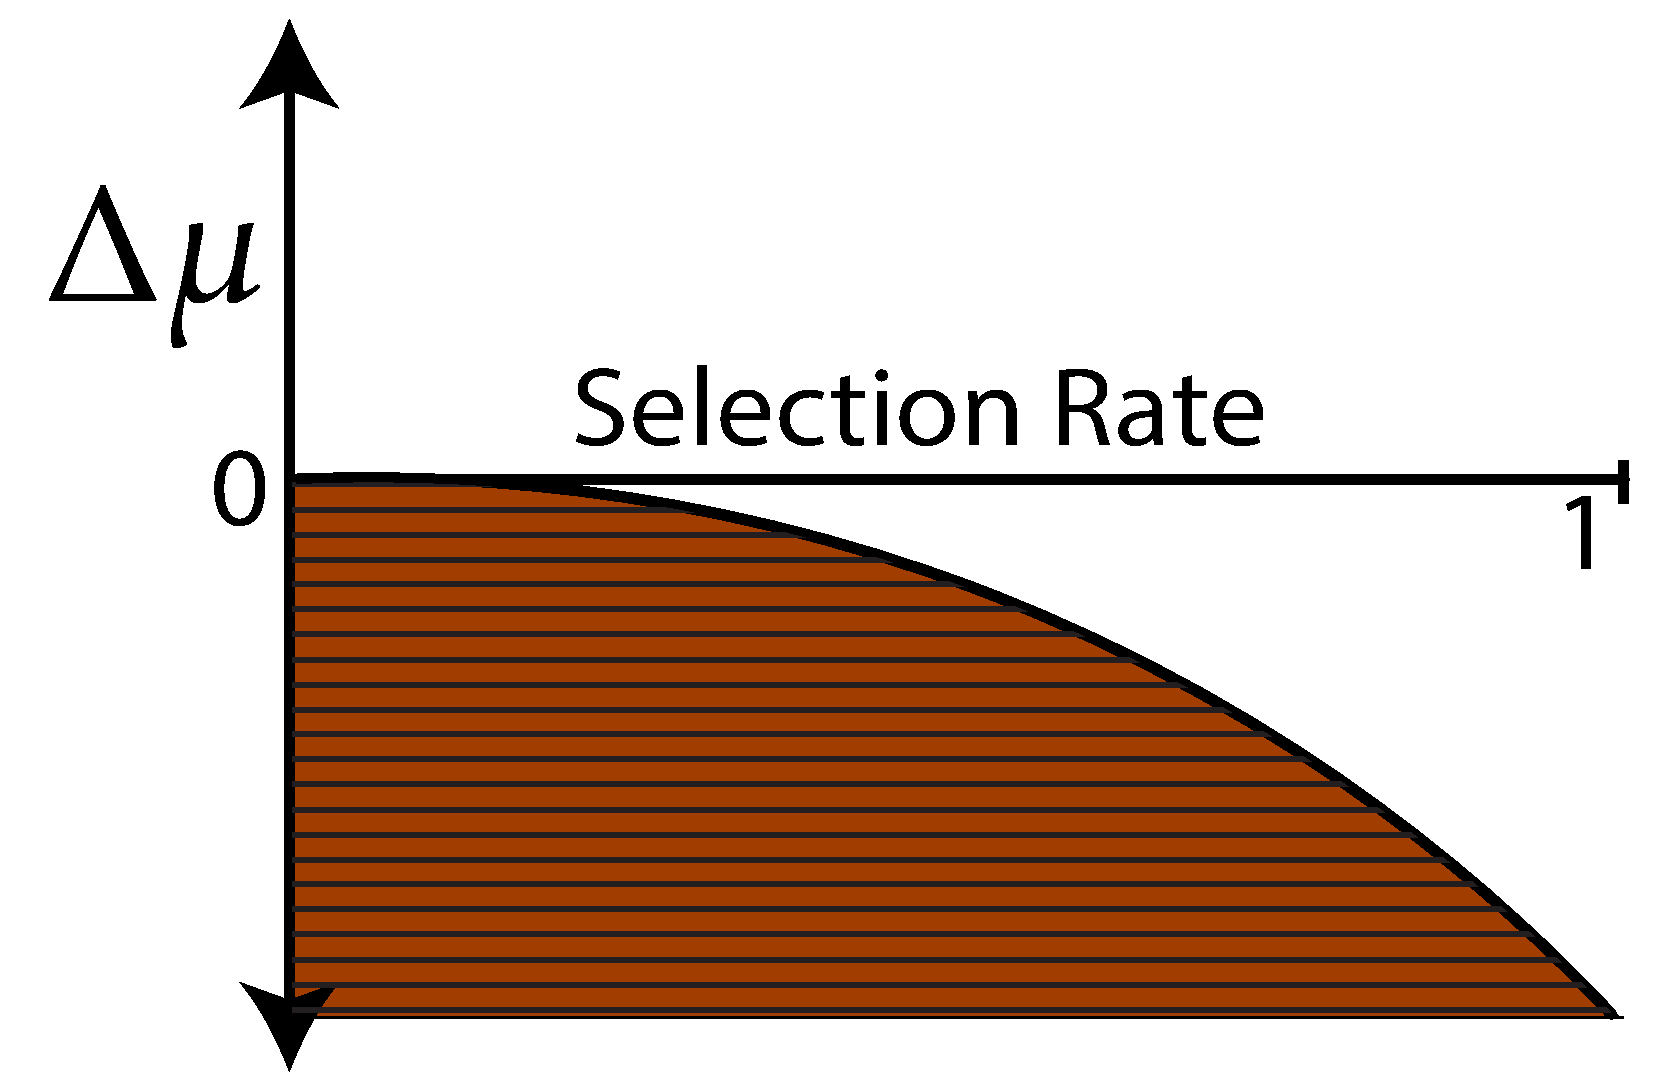
\includegraphics[width=\textwidth]{figures/outcome_curves/outcome_curve_bad.pdf}
\caption{}
\label{fig:sub2}
\end{subfigure}
\caption{The above figure shows the \emph{outcome curve}. The horizontal axis represents the selection rate for the population; the vertical axis represents the mean change in score. (a) depicts the full spectrum of outcome regimes, and colors indicate regions of active harm, relative harm, and no harm. In (b): a group that has much potential for gain, in (c): a group that has no potential for gain.}
\label{fig:outcome_curve}
\end{figure*}

Figure~\ref{fig:outcome_curve} displays the important outcome regimes in terms of \emph{selection rates} $\accrate\supj := \sum_{x \in \X} \distj(x)\polj(x)$. This succinct characterization is possible when considering decision rules based on (possibly randomized) score thresholding, in which all individuals with scores above a threshold are selected. In Section~\ref{section:opt_threshold}, we justify the restriction to such \emph{threshold policies} by showing it preserves optimality. In Section~\ref{section:concavity_outcome}, we show that the outcome curve is concave, thus implying that it takes the shape depicted in Figure~\ref{fig:outcome_curve}. To explicitly connect selection rates to decision policies, we define the rate function $\ratef_{\dist}(\polj)$ which returns the proportion of group $\popj$ selected by the policy. We show that this function is invertible for a suitable class of threshold policies, and in fact the outcome curve is precisely the graph of the map from selection rate to outcome $\accrate \mapsto \delmean\supa (\ratef_{\dista}^{-1}(\accrate))$. Next, we define the values of $\accrate$ that mark boundaries of the outcome regions.

\begin{defn}[Selection rates of interest]\label{def:special_betas}
	Given the protected group $\popa$, the following selection rates are of interest in distinguishing between qualitatively different classes of outcomes (Figure \ref{fig:outcome_curve}). We define $\accrate^{\maxprof}$ as the selection rate for $\popa$ under $\maxprof$; $\accrate_0$ as the harm threshold, such that $\delmean\supa(\ratef^{-1}_{\dista}(\accrate_0))~=~0$; $\accrate^*$ as the selection rate such that $\delmean\supa$ is maximized; $\overline{\accrate}$ as the outcome-complement of the $\maxprof$ selection rate, $\delmean\supa \ratef_{\dista}^{-1}(\overline{\accrate}))~=~\delmean\supa (\ratef_{\dista}^{-1}(\accrate^\maxprof))$ with $\overline{\accrate}~>~\accrate^{\maxprof}$.
\end{defn}



\subsection{Decision Rules and Fairness Criteria}
\label{sec:fairness_criteria}
We will consider policies that maximize the institution's total expected utility, potentially subject to a constraint: $\pol \in \Constraint \in [0,1]^{2\maxscore}$ which enforces some notion of ``fairness''. Formally, the institution selects $\tau_* \in \argmax~\Util(\pol) ~\subto~ \pol \in \Constraint$. We consider the three following constraints:
\begin{defn}[Fairness criteria] The \emph{maximum utility} ($\maxprof$) policy corresponds to the null-constraint $\Constraint = [0,1]^{2\maxscore}$, so that the institution is free to focus solely on utility. The \emph{demographic parity} ($\dempar$) policy results in equal selection rates between both groups. Formally, the constraint is
%\begin{eqnarray}
%\textstyle
$\Constraint = \left\{(\pola,\polb): \sum_{x \in \X} \dist\supa(x)\pola =
\sum_{x \in \X} \dist\supb(x)\polb\right\}\:.$
%\end{eqnarray}
The \emph{equal opportunity} ($\eqop$) policy results in equal true positive rates (TPR) between both group, where TPR is defined as $\oppj(\pol) :=\frac{\sum_{x \in \X} \dist\supj(x)\pb(x)\pol(x)}{\sum_{x \in \X} \dist\supj(x)\pb(x)}$.  $\eqop$ ensures that the conditional probability of selection given that the individual will be successful is independent of the population, formally enforced by the constraint
%\begin{eqnarray}
%\textstyle
$\Constraint = \left\{(\pola,\polb): \oppa(\pola) = \oppb(\polb) \right\}\,.$
%\end{eqnarray}
\end{defn}

Just as the expected outcome $\delmean$ can be expressed in terms of selection rate for threshold policies, so can the total utility $\Util$. In the unconstrained cause, $\Util$ varies independently over the selection rates for group $\popa$ and $\popb$; however, in the presence of fairness constraints the selection rate for one group determines the allowable selection rate for the other. The selection rates must be equal for $\dempar$, but for $\eqop$ we can define a \emph{transfer function}, $\transfer$, which for every loan rate $\beta$ in group $\popa$ gives the loan rate in group $\popb$ that has the same true positive rate. Therefore, when considering threshold policies, decision rules amount to maximizing functions of single parameters. This idea is expressed in Figure~\ref{fig:outcome_util_curves}, and underpins the results to follow.

